
%%%%%%%%%%%%%%%%%% PREAMBULE %%%%%%%%%%%%%%%%%%

\documentclass[aspectratio=169,utf8]{beamer}
%\documentclass[aspectratio=169,handout]{beamer}

\usetheme{Boadilla}
%\usecolortheme{seahorse}
\usecolortheme[RGB={245,66,24}]{structure}
\useoutertheme{infolines}

% packages
\usepackage{amsfonts,amsmath,amssymb,amsthm}
\usepackage[utf8]{inputenc}
\usepackage[T1]{fontenc}
\usepackage{lmodern}

\usepackage[francais]{babel}
\usepackage{fancybox}
\usepackage{graphicx}

\usepackage{float}
\usepackage{xfrac}

%\usepackage[usenames, x11names]{xcolor}
\usepackage{tikz}
\usepackage{pgfplots}
\usepackage{datetime}



%-----  Package unités -----
\usepackage{siunitx}
\sisetup{locale = FR,detect-all,per-mode = symbol}

%\usepackage{mathptmx}
%\usepackage{fouriernc}
%\usepackage{newcent}
%\usepackage[mathcal,mathbf]{euler}

%\usepackage{palatino}
%\usepackage{newcent}
% \usepackage[mathcal,mathbf]{euler}



% \usepackage{hyperref}
% \hypersetup{colorlinks=true, linkcolor=blue, urlcolor=blue,
% pdftitle={Exo7 - Exercices de mathématiques}, pdfauthor={Exo7}}


%section
% \usepackage{sectsty}
% \allsectionsfont{\bf}
%\sectionfont{\color{Tomato3}\upshape\selectfont}
%\subsectionfont{\color{Tomato4}\upshape\selectfont}

%----- Ensembles : entiers, reels, complexes -----
\newcommand{\Nn}{\mathbb{N}} \newcommand{\N}{\mathbb{N}}
\newcommand{\Zz}{\mathbb{Z}} \newcommand{\Z}{\mathbb{Z}}
\newcommand{\Qq}{\mathbb{Q}} \newcommand{\Q}{\mathbb{Q}}
\newcommand{\Rr}{\mathbb{R}} \newcommand{\R}{\mathbb{R}}
\newcommand{\Cc}{\mathbb{C}} 
\newcommand{\Kk}{\mathbb{K}} \newcommand{\K}{\mathbb{K}}

%----- Modifications de symboles -----
\renewcommand{\epsilon}{\varepsilon}
\renewcommand{\Re}{\mathop{\text{Re}}\nolimits}
\renewcommand{\Im}{\mathop{\text{Im}}\nolimits}
%\newcommand{\llbracket}{\left[\kern-0.15em\left[}
%\newcommand{\rrbracket}{\right]\kern-0.15em\right]}

\renewcommand{\ge}{\geqslant}
\renewcommand{\geq}{\geqslant}
\renewcommand{\le}{\leqslant}
\renewcommand{\leq}{\leqslant}
\renewcommand{\epsilon}{\varepsilon}

%----- Fonctions usuelles -----
\newcommand{\ch}{\mathop{\text{ch}}\nolimits}
\newcommand{\sh}{\mathop{\text{sh}}\nolimits}
\renewcommand{\tanh}{\mathop{\text{th}}\nolimits}
\newcommand{\cotan}{\mathop{\text{cotan}}\nolimits}
\newcommand{\Arcsin}{\mathop{\text{arcsin}}\nolimits}
\newcommand{\Arccos}{\mathop{\text{arccos}}\nolimits}
\newcommand{\Arctan}{\mathop{\text{arctan}}\nolimits}
\newcommand{\Argsh}{\mathop{\text{argsh}}\nolimits}
\newcommand{\Argch}{\mathop{\text{argch}}\nolimits}
\newcommand{\Argth}{\mathop{\text{argth}}\nolimits}
\newcommand{\pgcd}{\mathop{\text{pgcd}}\nolimits} 


%----- Commandes divers ------
\newcommand{\ii}{\mathrm{i}}
\newcommand{\dd}{\text{d}}
\newcommand{\id}{\mathop{\text{id}}\nolimits}
\newcommand{\Ker}{\mathop{\text{Ker}}\nolimits}
\newcommand{\Card}{\mathop{\text{Card}}\nolimits}
\newcommand{\Vect}{\mathop{\text{Vect}}\nolimits}
\newcommand{\Mat}{\mathop{\text{Mat}}\nolimits}
\newcommand{\rg}{\mathop{\text{rg}}\nolimits}
\newcommand{\tr}{\mathop{\text{tr}}\nolimits}


%----- Structure des exercices ------

\newtheoremstyle{styleexo}% name
{2ex}% Space above
{3ex}% Space below
{}% Body font
{}% Indent amount 1
{\bfseries} % Theorem head font
{}% Punctuation after theorem head
{\newline}% Space after theorem head 2
{}% Theorem head spec (can be left empty, meaning ‘normal’)

%\theoremstyle{styleexo}
\newtheorem{exo}{Exercice}
\newtheorem{ind}{Indications}
\newtheorem{cor}{Correction}


\newcommand{\exercice}[1]{} \newcommand{\finexercice}{}
%\newcommand{\exercice}[1]{{\tiny\texttt{#1}}\vspace{-2ex}} % pour afficher le numero absolu, l'auteur...
\newcommand{\enonce}{\begin{exo}} \newcommand{\finenonce}{\end{exo}}
\newcommand{\indication}{\begin{ind}} \newcommand{\finindication}{\end{ind}}
\newcommand{\correction}{\begin{cor}} \newcommand{\fincorrection}{\end{cor}}

\newcommand{\noindication}{\stepcounter{ind}}
\newcommand{\nocorrection}{\stepcounter{cor}}

\newcommand{\fiche}[1]{} \newcommand{\finfiche}{}
\newcommand{\titre}[1]{\centerline{\large \bf #1}}
\newcommand{\addcommand}[1]{}
\newcommand{\video}[1]{}

% Marge
\newcommand{\mymargin}[1]{\marginpar{{\small #1}}}

\def\noqed{\renewcommand{\qedsymbol}{}}


%----- Presentation ------
\setlength{\parindent}{0cm}

%\newcommand{\ExoSept}{\href{http://exo7.emath.fr}{\textbf{\textsf{Exo7}}}}

\definecolor{myred}{rgb}{0.93,0.26,0}
\definecolor{myorange}{rgb}{0.97,0.58,0}
\definecolor{myyellow}{rgb}{1,0.86,0}

\newcommand{\LogoExoSept}[1]{  % input : echelle
{\usefont{U}{cmss}{bx}{n}
\begin{tikzpicture}[scale=0.1*#1,transform shape]
  \fill[color=myorange] (0,0)--(4,0)--(4,-4)--(0,-4)--cycle;
  \fill[color=myred] (0,0)--(0,3)--(-3,3)--(-3,0)--cycle;
  \fill[color=myyellow] (4,0)--(7,4)--(3,7)--(0,3)--cycle;
  \node[scale=5] at (3.5,3.5) {Exo7};
\end{tikzpicture}}
}


\newcommand{\debutmontitre}{
  \author{} \date{} 
  \thispagestyle{empty}
  \hspace*{-10ex}
  \begin{minipage}{\textwidth}
    \titlepage  
  \vspace*{-2.5cm}
  \begin{center}
    \LogoExoSept{2.5}
  \end{center}
  \end{minipage}

  \vspace*{-0cm}
  
  % Astuce pour que le background ne soit pas discrétisé lors de la conversion pdf -> png
\begin{tikzpicture}
        \fill[opacity=0,green!60!black] (0,0)--++(0,0)--++(0,0)--++(0,0)--cycle; 
\end{tikzpicture}

% toc S'affiche trop tot :
% \tableofcontents[hideallsubsections, pausesections]
}

\newcommand{\finmontitre}{
  \end{frame}
  \setcounter{framenumber}{0}
} % ne marche pas pour une raison obscure

%----- Commandes supplementaires ------

% \usepackage[landscape]{geometry}
% \geometry{top=1cm, bottom=3cm, left=2cm, right=10cm, marginparsep=1cm
% }
% \usepackage[a4paper]{geometry}
% \geometry{top=2cm, bottom=2cm, left=2cm, right=2cm, marginparsep=1cm
% }

%\usepackage{standalone}


% New command Arnaud -- november 2011
\setbeamersize{text margin left=24ex}
% si vous modifier cette valeur il faut aussi
% modifier le decalage du titre pour compenser
% (ex : ici =+10ex, titre =-5ex

\theoremstyle{definition}
%\newtheorem{proposition}{Proposition}
%\newtheorem{exemple}{Exemple}
%\newtheorem{theoreme}{Théorème}
%\newtheorem{lemme}{Lemme}
%\newtheorem{corollaire}{Corollaire}
%\newtheorem*{remarque*}{Remarque}
%\newtheorem*{miniexercice}{Mini-exercices}
%\newtheorem{definition}{Définition}

% Commande tikz
\usetikzlibrary{calc}
\usetikzlibrary{patterns,arrows}
\usetikzlibrary{matrix}
\usetikzlibrary{fadings} 

%definition d'un terme
\newcommand{\defi}[1]{{\color{myorange}\textbf{\emph{#1}}}}
\newcommand{\evidence}[1]{{\color{blue}\textbf{\emph{#1}}}}
\newcommand{\assertion}[1]{\emph{\og#1\fg}}  % pour chapitre logique
%\renewcommand{\contentsname}{Sommaire}
\renewcommand{\contentsname}{}
\setcounter{tocdepth}{2}



%------ Figures ------

\def\myscale{1} % par défaut 
\newcommand{\myfigure}[2]{  % entrée : echelle, fichier figure
\def\myscale{#1}
\begin{center}
\footnotesize
{#2}
\end{center}}


%------ Encadrement ------

\usepackage{fancybox}


\newcommand{\mybox}[1]{
\setlength{\fboxsep}{7pt}
\begin{center}
\shadowbox{#1}
\end{center}}

\newcommand{\myboxinline}[1]{
\setlength{\fboxsep}{5pt}
\raisebox{-10pt}{
\shadowbox{#1}
}
}

%--------------- Commande beamer---------------
\newcommand{\beameronly}[1]{#1} % permet de mettre des pause dans beamer pas dans poly


\setbeamertemplate{navigation symbols}{}
\setbeamertemplate{footline}  % tiré du fichier beamerouterinfolines.sty
{
  \leavevmode%
  \hbox{%
  \begin{beamercolorbox}[wd=.333333\paperwidth,ht=2.25ex,dp=1ex,center]{author in head/foot}%
    % \usebeamerfont{author in head/foot}\insertshortauthor%~~(\insertshortinstitute)
    \usebeamerfont{section in head/foot}{\bf\insertshorttitle}
  \end{beamercolorbox}%
  \begin{beamercolorbox}[wd=.333333\paperwidth,ht=2.25ex,dp=1ex,center]{title in head/foot}%
    \usebeamerfont{section in head/foot}{\bf\insertsectionhead}
  \end{beamercolorbox}%
  \begin{beamercolorbox}[wd=.333333\paperwidth,ht=2.25ex,dp=1ex,right]{date in head/foot}%
    % \usebeamerfont{date in head/foot}\insertshortdate{}\hspace*{2em}
    \insertframenumber{} / \inserttotalframenumber\hspace*{2ex} 
  \end{beamercolorbox}}%
  \vskip0pt%
}


\definecolor{mygrey}{rgb}{0.5,0.5,0.5}
\setlength{\parindent}{0cm}
%\DeclareTextFontCommand{\helvetica}{\fontfamily{phv}\selectfont}

% background beamer
\definecolor{couleurhaut}{rgb}{0.85,0.9,1}  % creme
\definecolor{couleurmilieu}{rgb}{1,1,1}  % vert pale
\definecolor{couleurbas}{rgb}{0.85,0.9,1}  % blanc
\setbeamertemplate{background canvas}[vertical shading]%
[top=couleurhaut,middle=couleurmilieu,midpoint=0.4,bottom=couleurbas] 
%[top=fondtitre!05,bottom=fondtitre!60]



\makeatletter
\setbeamertemplate{theorem begin}
{%
  \begin{\inserttheoremblockenv}
  {%
    \inserttheoremheadfont
    \inserttheoremname
    \inserttheoremnumber
    \ifx\inserttheoremaddition\@empty\else\ (\inserttheoremaddition)\fi%
    \inserttheorempunctuation
  }%
}
\setbeamertemplate{theorem end}{\end{\inserttheoremblockenv}}

\newenvironment{theoreme}[1][]{%
   \setbeamercolor{block title}{fg=structure,bg=structure!40}
   \setbeamercolor{block body}{fg=black,bg=structure!10}
   \begin{block}{{\bf Th\'eor\`eme }#1}
}{%
   \end{block}%
}


\newenvironment{proposition}[1][]{%
   \setbeamercolor{block title}{fg=structure,bg=structure!40}
   \setbeamercolor{block body}{fg=black,bg=structure!10}
   \begin{block}{{\bf Proposition }#1}
}{%
   \end{block}%
}

\newenvironment{corollaire}[1][]{%
   \setbeamercolor{block title}{fg=structure,bg=structure!40}
   \setbeamercolor{block body}{fg=black,bg=structure!10}
   \begin{block}{{\bf Corollaire }#1}
}{%
   \end{block}%
}

\newenvironment{mydefinition}[1][]{%
   \setbeamercolor{block title}{fg=structure,bg=structure!40}
   \setbeamercolor{block body}{fg=black,bg=structure!10}
   \begin{block}{{\bf Définition} #1}
}{%
   \end{block}%
}

\newenvironment{lemme}[0]{%
   \setbeamercolor{block title}{fg=structure,bg=structure!40}
   \setbeamercolor{block body}{fg=black,bg=structure!10}
   \begin{block}{\bf Lemme}
}{%
   \end{block}%
}

\newenvironment{remarque}[1][]{%
   \setbeamercolor{block title}{fg=black,bg=structure!20}
   \setbeamercolor{block body}{fg=black,bg=structure!5}
   \begin{block}{Remarque #1}
}{%
   \end{block}%
}


\newenvironment{exemple}[1][]{%
   \setbeamercolor{block title}{fg=black,bg=structure!20}
   \setbeamercolor{block body}{fg=black,bg=structure!5}
   \begin{block}{{\bf Exemple }#1}
}{%
   \end{block}%
}


\newenvironment{miniexercice}[0]{%
   \setbeamercolor{block title}{fg=structure,bg=structure!20}
   \setbeamercolor{block body}{fg=black,bg=structure!5}
   \begin{block}{Mini-exercices}
}{%
   \end{block}%
}


\newenvironment{tp}[0]{%
   \setbeamercolor{block title}{fg=structure,bg=structure!40}
   \setbeamercolor{block body}{fg=black,bg=structure!10}
   \begin{block}{\bf Travaux pratiques}
}{%
   \end{block}%
}
\newenvironment{exercicecours}[1][]{%
   \setbeamercolor{block title}{fg=structure,bg=structure!40}
   \setbeamercolor{block body}{fg=black,bg=structure!10}
   \begin{block}{{\bf Exercice }#1}
}{%
   \end{block}%
}
\newenvironment{algo}[1][]{%
   \setbeamercolor{block title}{fg=structure,bg=structure!40}
   \setbeamercolor{block body}{fg=black,bg=structure!10}
   \begin{block}{{\bf Algorithme}\hfill{\color{gray}\texttt{#1}}}
}{%
   \end{block}%
}


\setbeamertemplate{proof begin}{
   \setbeamercolor{block title}{fg=black,bg=structure!20}
   \setbeamercolor{block body}{fg=black,bg=structure!5}
   \begin{block}{{\footnotesize Démonstration}}
   \footnotesize
   \smallskip}
\setbeamertemplate{proof end}{%
   \end{block}}
\setbeamertemplate{qed symbol}{\openbox}


\makeatother
\usecolortheme[RGB={0,0,102}]{structure}
   
%%%%%%%%%%%%%%%%%%%%%%%%%%%%%%%%%%%%%%%%%%%%%%%%%%%%%%%%%%%%%
%%%%%%%%%%%%%%%%%%%%%%%%%%%%%%%%%%%%%%%%%%%%%%%%%%%%%%%%%%%%%


\begin{document}


\title{{\bf La chaînette}}
\subtitle{Longueur d'une chaînette}

\begin{frame}
  
  \debutmontitre

  \pause

{\footnotesize
\hfill
\setbeamercovered{transparent=50}
\begin{minipage}{0.6\textwidth}
  \begin{itemize}
    \item<3-> Longueur d'une chaînette
    \item<4-> Calcul du paramètre
    \item<5-> \'Equation paramétrique
    \item<6-> Calcul de la tension
    \item<7-> Exercices
  \end{itemize}
\end{minipage}
}

\end{frame}

\setcounter{framenumber}{0}


%%%%%%%%%%%%%%%%%%%%%%%%%%%%%%%%%%%%%%%%%%%%%%%%%%%%%%%%%%%%%%%%
\section{Longueur d'une chaînette}

\begin{frame}
\begin{proposition}
\label{prop:long}
La longueur de la portion de la chaînette de paramètre $a$ entre le point le plus 
bas $(0,a)$ et le point d'abscisse $x_0$ est :
$$\ell = a \sh \frac{x_0}{a}$$
\end{proposition}
\shorthandoff{:}
\myfigure{1}{
\tikzinput{fig_chainette17}
}
\shorthandon{:}
\end{frame}


\begin{frame}
\begin{proof}
\begin{itemize}

  \uncover<2->{\item L'équation de la chaînette : $y(x) =a \ch \frac x a$}
  \uncover<3->{\item La longueur vaut $\ell = \int_0^{x_0} \sqrt{1+y'(x)^2} dx$}
\end{itemize}
\vspace*{-1ex}
$$\begin{array}{rcl}
 \uncover<4->{\ell 
   &=& \int_0^{x_0} \sqrt{1+\sh^2 \tfrac x a} dx \quad \text{ car } \ch' \tfrac x a = \frac 1 a \sh \tfrac x a \\[2mm]}
   \uncover<5->{&=& \int_0^{x_0} \sqrt{\ch^2 \tfrac x a} dx   \quad \text{ car } 1+\sh^2 u = \ch^2 u \\[2mm]}
   \uncover<6->{&=& \int_0^{x_0} \ch \tfrac x a dx \\[2mm]}
   \uncover<7->{&=&  \left[ a \sh \tfrac x a \right]_0^{x_0} \\[2mm]}
   \uncover<8->{&=& a \sh \tfrac{x_0}{a}}
\end{array}$$

\vspace*{-1ex}
\end{proof}
\shorthandoff{:}
\myfigure{0.8}{
\tikzinput{fig_chainette17}
}
\shorthandon{:}
\end{frame}

%%%%%%%%%%%%%%%%%%%%%%%%%%%%%%%%%%%%%%%%%%%%%%%%%%%%%%%%%%%%%%%%
\section{Calcul du paramètre}

\begin{frame}

\begin{itemize}
  \uncover<2->{\item La chaînette ne dépend que du seul paramètre $a$}
  
  \uncover<3->{\item $a = \frac{T_h}{\mu g}$}
  
  \uncover<4->{\item Prenons une chaînette de longueur $2\ell$ fixée}
  
  \uncover<5->{\item La \defi{flèche} est la hauteur $h$ entre les deux points d'accroche
et le point le plus bas de la chaînette}
\end{itemize}

\shorthandoff{:}
\myfigure{1.3}{
\tikzinput{fig_chainette11}
}
\shorthandon{:}
\end{frame}


\begin{frame}
\begin{proposition}
\label{prop:param}
\begin{minipage}{0.5\textwidth}
Pour une chaînette de longueur $2\ell$ et de flèche $h$ alors
$$a=\frac{\ell^2-h^2}{2h}$$
\end{minipage}\quad
\begin{minipage}{0.29\textwidth}
\shorthandoff{:}
\myfigure{0.8}{
\tikzinput{fig_chainette11}
}
\shorthandon{:}  
\end{minipage}\vspace*{-1ex}
\end{proposition}
\pause
\begin{proof}\vspace*{-1ex}
\begin{itemize}
  \item $(\pm x_0, y_0)$ les coordonnées des points d'accroche
  \pause
  \item $y_0 = a \ch \frac{x_0}{a} = a + h$ \pause \ donc $h = a \ch \frac{x_0}{a} -a$
  \pause
  \item $\ell =  a \sh \left( \frac{x_0}{a} \right)$
\end{itemize}
\vspace*{-2ex}
\pause
$$\begin{array}{rcl}
\ell^2 - h^2 
  \pause &=& a^2 \sh^2 \tfrac{x_0}{a} - \left( a \ch \tfrac{x_0}{a} - a \right)^2 \\
  \pause &=& a^2 \sh^2 \tfrac{x_0}{a} - a^2 \ch^2  \tfrac{x_0}{a} -a^2 +2 a^2 \ch \tfrac{x_0}{a} \\
  \pause &=& 2a\left(-a+a \ch \tfrac{x_0}{a} \right) \qquad \text{ car } \ch^2 u - \sh^2 u = 1 \\
  \pause &=& 2ah \\
\end{array}$$
\vspace*{-2ex}

\pause
Ainsi \ \ $a = \displaystyle\frac{\ell^2-h^2}{2h}$
\end{proof}
\end{frame}




%%%%%%%%%%%%%%%%%%%%%%%%%%%%%%%%%%%%%%%%%%%%%%%%%%%%%%%%%%%%%%%%
\section{\'Equation paramétrique}

\begin{frame}
\begin{proposition}
Une équation paramétrique de la chaînette est :
$$\left\{
\begin{array}{rcl}
x(t) &=& a \ln t \\
y(t) &=& \frac a 2 \left(t+\frac 1 t\right)
\end{array}
\right.
$$
pour $t>0$
\end{proposition}

\end{frame}



%%%%%%%%%%%%%%%%%%%%%%%%%%%%%%%%%%%%%%%%%%%%%%%%%%%%%%%%%%%%%%%%
\section{Calcul de la tension}

\begin{frame}
\begin{proposition}
\label{prop:tens}
\begin{itemize}
\setlength{\itemsep}{5pt}
  \uncover<2->{\item La \evidence{tension horizontale} $T_h$ est constante 
  $\displaystyle T_h = a \mu g = \frac{\ell^2-h^2}{2h} \mu g$}
  
  \uncover<3->{\item Le \evidence{tension verticale} 
  $\displaystyle T_v= T_h \cdot \sh \frac{x_0}{a} = T_h \cdot \frac \ell a$}
  
  \uncover<4->{\item La \evidence{tension totale} 
  $\displaystyle T = \sqrt{T_h^2+T_v^2} = T_h \cdot \ch \frac{x_0}{a} = T_h \cdot \frac{a+h}{a}$}
\end{itemize}
\shorthandoff{:}
\myfigure{0.8}{
\tikzinput{fig_chainette12}
}
\shorthandon{:}
\vspace*{-2ex}

\end{proposition}
\end{frame}


\begin{frame}

\begin{proof}
\hfill \begin{minipage}{0.40\textwidth}
\shorthandoff{:}
\myfigure{0.65}{
\tikzinput{fig_chainette12}
}
\shorthandon{:}  
\end{minipage}

\pause
\vspace*{-20ex}
\begin{itemize}
  \item \evidence{Tension horizontale}
  \pause
  \begin{itemize}
    \item La tension horizontale est constante
    \pause
    \item $T_h = a \mu g$ par définition de $a$
    \pause
    \item $T_h = \frac{\ell^2-h^2}{2h} \mu g$
  \end{itemize}
  
  \pause
  \item \evidence{Tension verticale}
  \pause
   \begin{itemize}
     \item $T_v(x_0) = T_h \cdot y'(x_0) =
  T_h \cdot \sh \frac{x_0}{a} = T_h \cdot \frac \ell a$
  \end{itemize}
 
 \pause
  \item \evidence{Tension totale}
  \begin{itemize} 
  \pause
    \item $\vec T(x) = -T_h(x)\vec i - T_v(x) \vec j$
    \pause
    \item $T(x_0) = \|\vec T(x_0) \|   = \sqrt{T_h^2+T_v^2(x_0)}$
  \pause
   \item $T(x_0) = T_h \sqrt{1+\sh^2 \frac{x_0}{a}}
  = T_h \cdot \ch \frac{x_0}{a} = T_h \cdot \frac{a+h}{a}$
   
  \end{itemize}
\end{itemize}

\end{proof}
\end{frame}


%%%%%%%%%%%%%%%%%%%%%%%%%%%%%%%%%%%%%%%%%%%%%%%%%%%%%%%%%%%%%%%%
\section{Exercices}

\begin{frame}


\begin{minipage}{0.49\textwidth}
\evidence{Tension minimale}
\begin{center}
   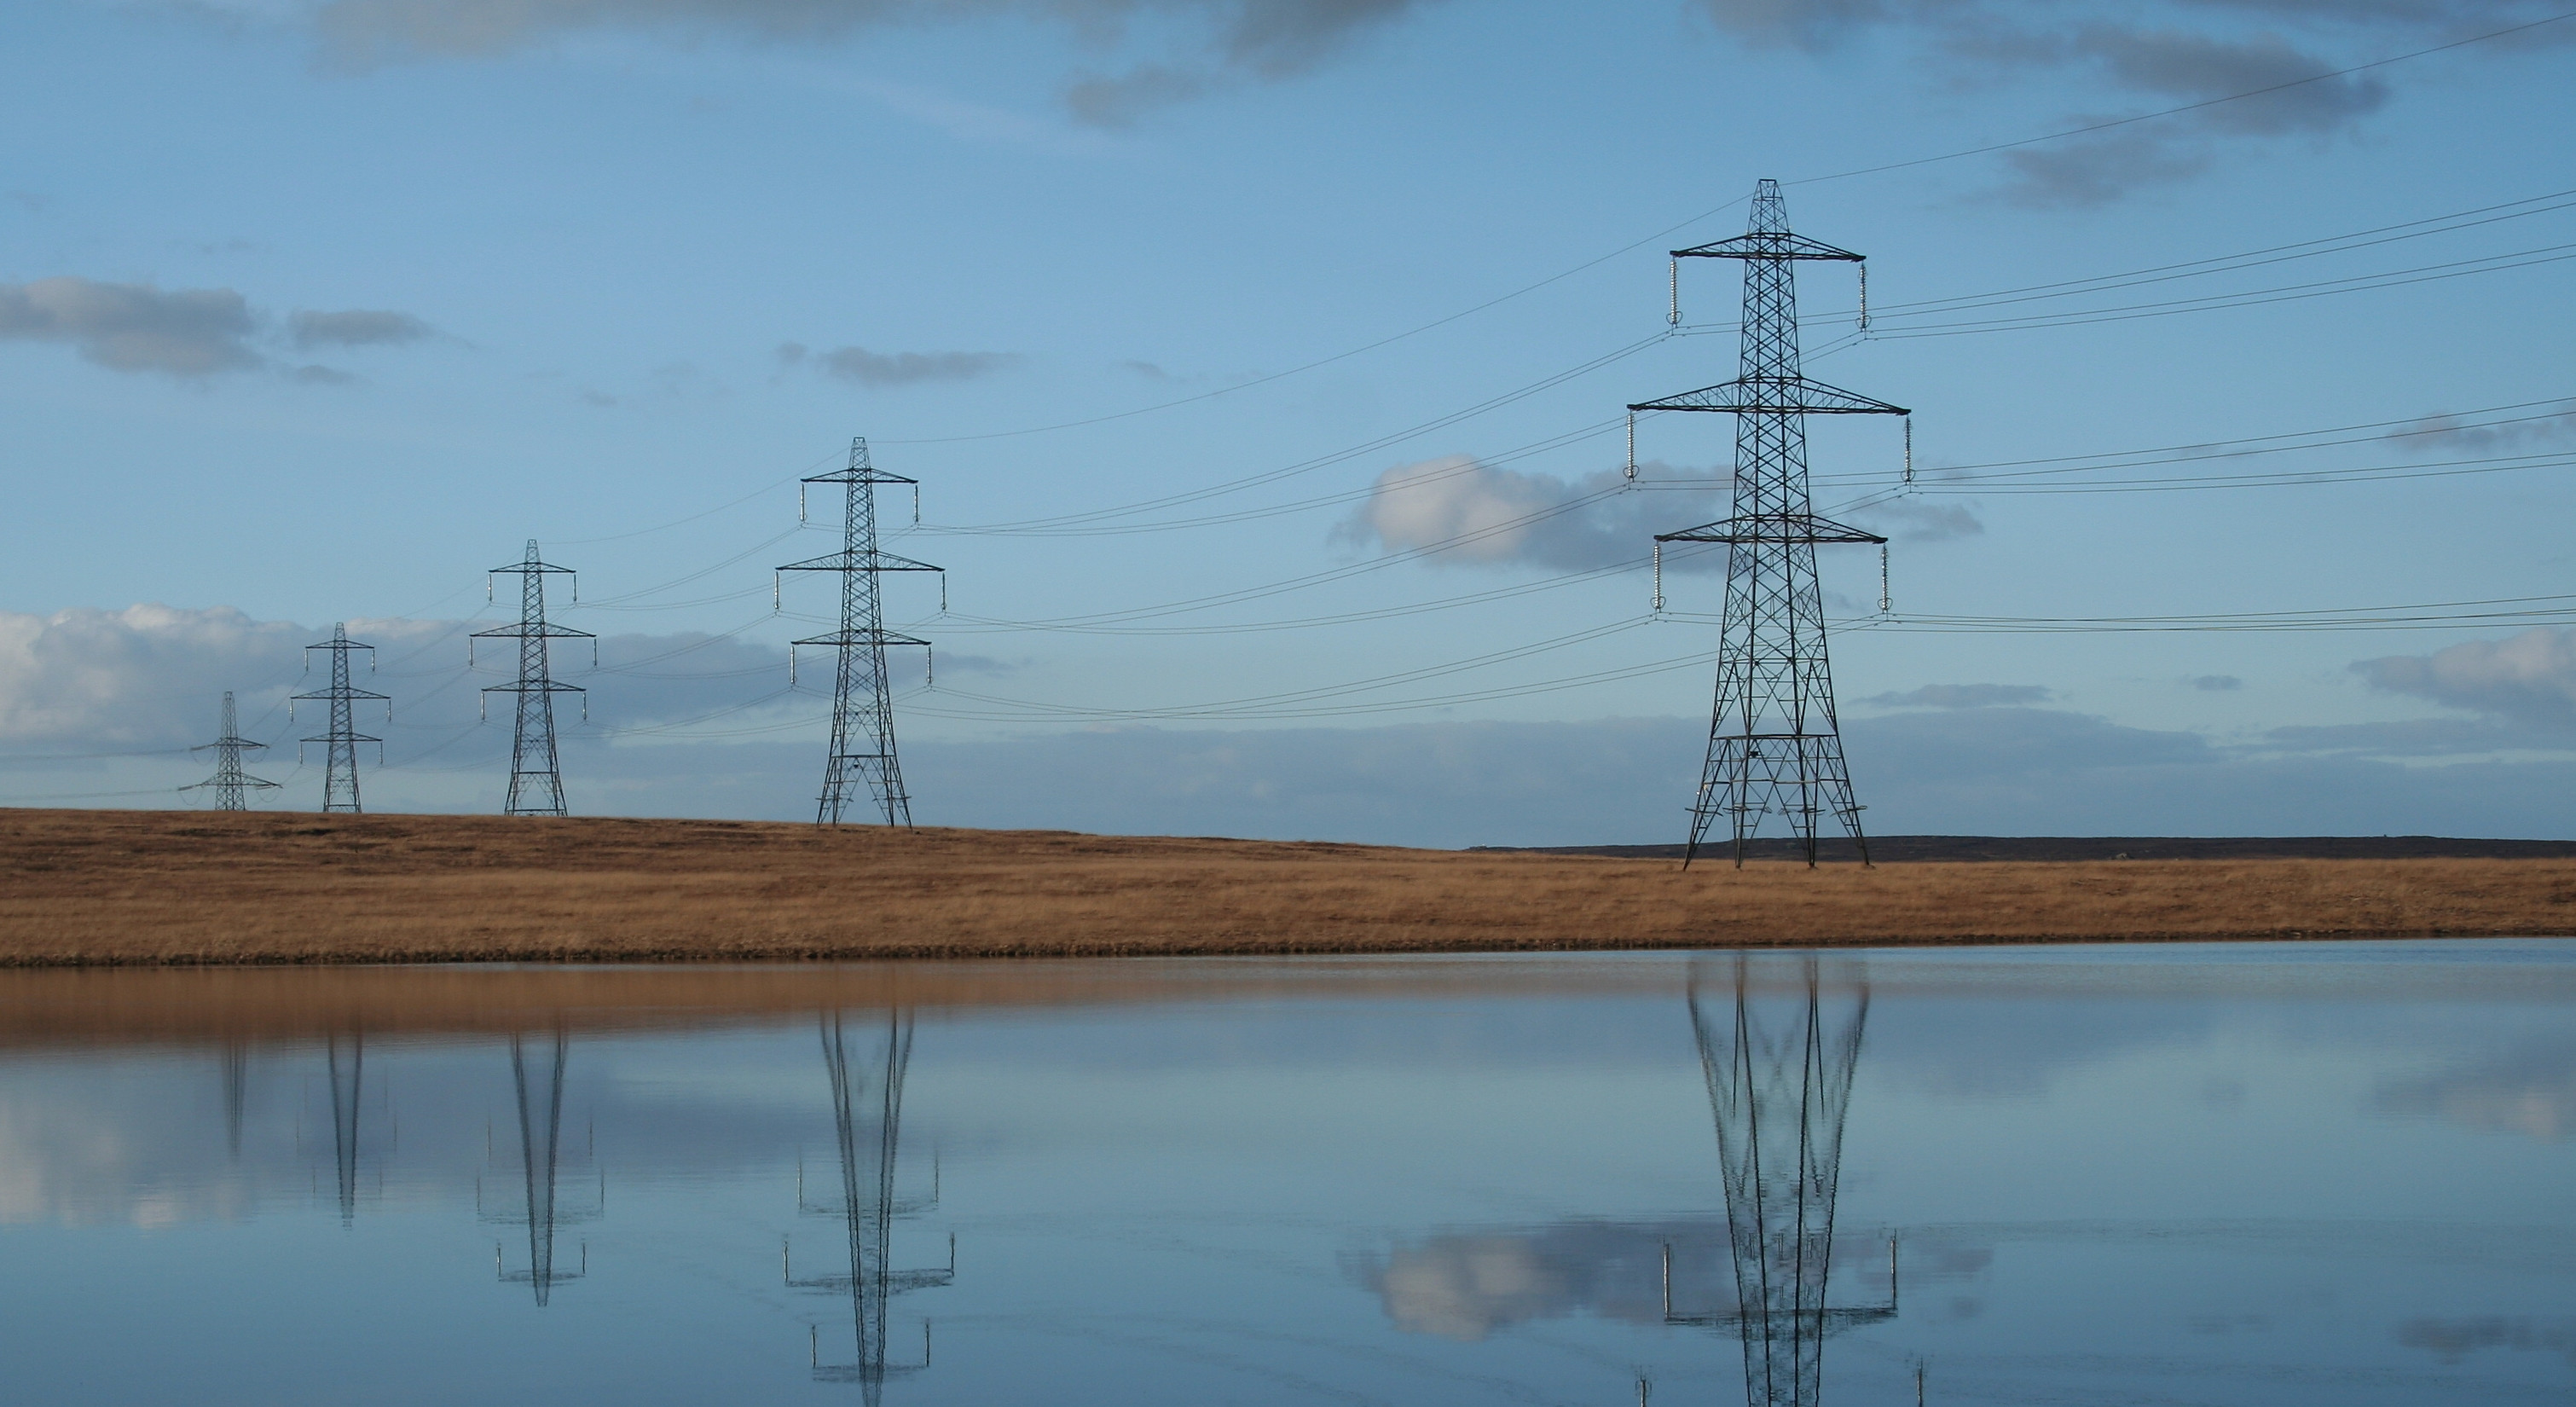
\includegraphics[width=\textwidth]{figures/Pylones_by_Graham_Sivills.jpg} 
 \end{center}  
\end{minipage}
\begin{minipage}{0.49\textwidth}
\shorthandoff{:}
\myfigure{0.7}{
\tikzinput{fig_chainette13}
}
\shorthandon{:}  
\end{minipage}

  \pause
 \begin{itemize}
   \item Deux poteaux distants d'une longueur $2x_0$ fixée
   \pause
   \item On cherche la chaînette ayant les forces de tensions minimales
   \pause
   \item La tension totale est 
   \vspace*{-2ex}
$$T_x(a) = a \mu g \cdot \ch \frac{x}{a}$$
 \vspace*{-4ex}
 \pause
  \item Tension maximale au point d'accroche (en $x=x_0$)
  \pause
  \item Pour un $a$ fixé, la tension maximale est donc $T_{x_0}(a)$
  \pause
  \item Problème : pour $x_0$ fixé, trouver le $a$ qui minimise $T_{x_0}(a)$
 \end{itemize}


\end{frame}


\begin{frame}
\begin{exercicecours}[Tension minimale]
\begin{enumerate}
 \item Considérations physiques : Que vaut la tension si la chaînette est rectiligne (la longueur de la chaînette
est celle de l'écartement) ? Que vaut la tension si la longueur de la chaînette est infinie ?
%% Dans les deux cas la tension est infinie, cela peut se montrer aussi par les calculs.

 \item Montrer que l'équation $\ch t = t \sh t$ est équivalente à l'équation 
$(t-1)e^{2t}=t+1$. Montrer que, sur $[0,+\infty[$, cette équation a une unique solution $\tau$.
Une valeur approchée de $\tau$ est $\tau = 1,19968\ldots$

%% $f(t) = (t-1)e^{2t}-t-1$, $f'(t) = (2t-1)e^{2t}-1$, $f''(t) = 4te^{2t}$.
% Poutr $t>0$, $f''(t)>0$ donc $f'$ strictement croissante.
% Or $f'(0)=-2$ le limite de $f'$ est $+\infty$ est $+\infty$. 
% Donc $f'$ s'annule en une seule valeur $\tau'$.
% Sur $[0,\tau']$, $f$ est décroissante, sur $[\tau', +\infty[$, $f$ est croissante.
% Comme $f(0) = -2 <0$ il n'y a pas de solution $f(t)=0$ sur $[0,\tau']$.
% Par le théorème des valeurs intermédiaires il existe un unique $\tau \in [\tau', +\infty[$
% tel que $f(\tau)=0$.

 \item Montrer que la tension $T_{x_0}(a)$ est minimale en $a= \frac{x_0}{\tau}$.

% $T'(a) = \mu g \left( \ch\frac{x_0}{a} - \frac{x_0}{a}\sh\frac{x_0}{a} \right)$
% S'annule en $\frac{x_0}{a} = \tau$ uniquement.
% Par les considérations physiques ce point est le minimum !

 \item Calculer la longueur correspondante, ainsi que la flèche.
\shorthandoff{:}
\myfigure{0.8}{
\tikzinput{fig_chainette14}
}
\shorthandon{:}
% $\ell = a \sh\frac{x_0}{a}  = \frac{x_0}{\tau} \sh \tau$
% $h = a \ch\frac{x_0}{a}  - a = \frac{x_0}{\tau} \ch \tau  - \frac{x_0}{\tau}$

\end{enumerate}

\end{exercicecours}

\end{frame}



\begin{frame}

\evidence{Pont suspendu}

\begin{itemize}
  \uncover<2->{\item La courbe du câble d'un pont suspendu
est une parabole}

  \uncover<3->{\item Le tablier d'un pont a une longueur $L$ et une masse totale $M$}
  
  \uncover<4->{\item Un gros câble est accroché entre deux pylônes}
  
  \uncover<5->{\item Ce câble est relié au tablier par des petits câbles de suspension}
  
  \uncover<6->{\item But : calculer l'équation du gros câble}
\end{itemize}


\shorthandoff{:}
\myfigure{1}{
\tikzinput{fig_chainette15}
}
\shorthandon{:}
\end{frame}



\begin{frame}
\begin{exercicecours}[Pont suspendu]
\begin{enumerate}

 \item Quelles sont les forces qui s'appliquent à une portion de câble dont l'abscisse est entre
 $x$ et $x+dx$ ?

% Quatre forces : $T(x)$, $-T(x+dx)$, $P(x)$, et la charge $C = Mg/L.dx$ dirigée vers le bas.

 \item \'Ecrire l'équation du principe fondamental de la mécanique, appliqué à cette portion.

% idem chainette + charge 

 \item Montrer que la tension horizontale est indépendante de $x$.

% idem chainette

 \item Montrer que la tension verticale vérifie l'équation différentielle :
$T'_v(x)=-T_h \cdot y''(x)$.

% idem chainette

 \item Dans toute la suite nous supposerons que la masse du câble est négligeable devant
celle du tablier. Cela revient à supposer que le poids $P(x)$ du câble est négligeable devant
la charge $C(x)$ du tablier. Nous posons donc $P(x)=0$.
Montrer que le principe fondamental de la mécanique s'écrit alors :
\vspace*{-2ex}
$$T_h \cdot y''(x) = \frac{M}{L} g.$$
\vspace*{-4ex}
% facile, ressemble chainette

 \item Quelle est l'équation $y(x)$ du câble ?

% Parabole
\end{enumerate}

\end{exercicecours}
\end{frame}


\begin{frame}



\begin{exercicecours}[Pont suspendu]

\begin{enumerate}
 \setcounter{enumi}{6}


 \item Calculer une équation du câble du \emph{Golden Bridge} (San Francisco).
Le tablier mesure $1280$ mètres de long, les pylônes ont une hauteur de $160$ mètres (au-dessus
du tablier) et le câble descend jusqu'au tablier (au milieu du pont).

\vspace*{-1ex}
\shorthandoff{:}
\myfigure{0.8}{
\tikzinput{fig_chainette16}
}
\shorthandon{:}


% Repère adapté : unité le mètre, (O,i,j) : O milieu du pont, i horizontal, j vertical.
% y = ax^2+bx + c
% y(0)=0 donc c=0, 
% par symetrie (principe physique) y(-x)=y(x) donc b=0
% y = ax^2 avec a = 160 / (1280/2)^2.
\end{enumerate}

\end{exercicecours}

\begin{center}
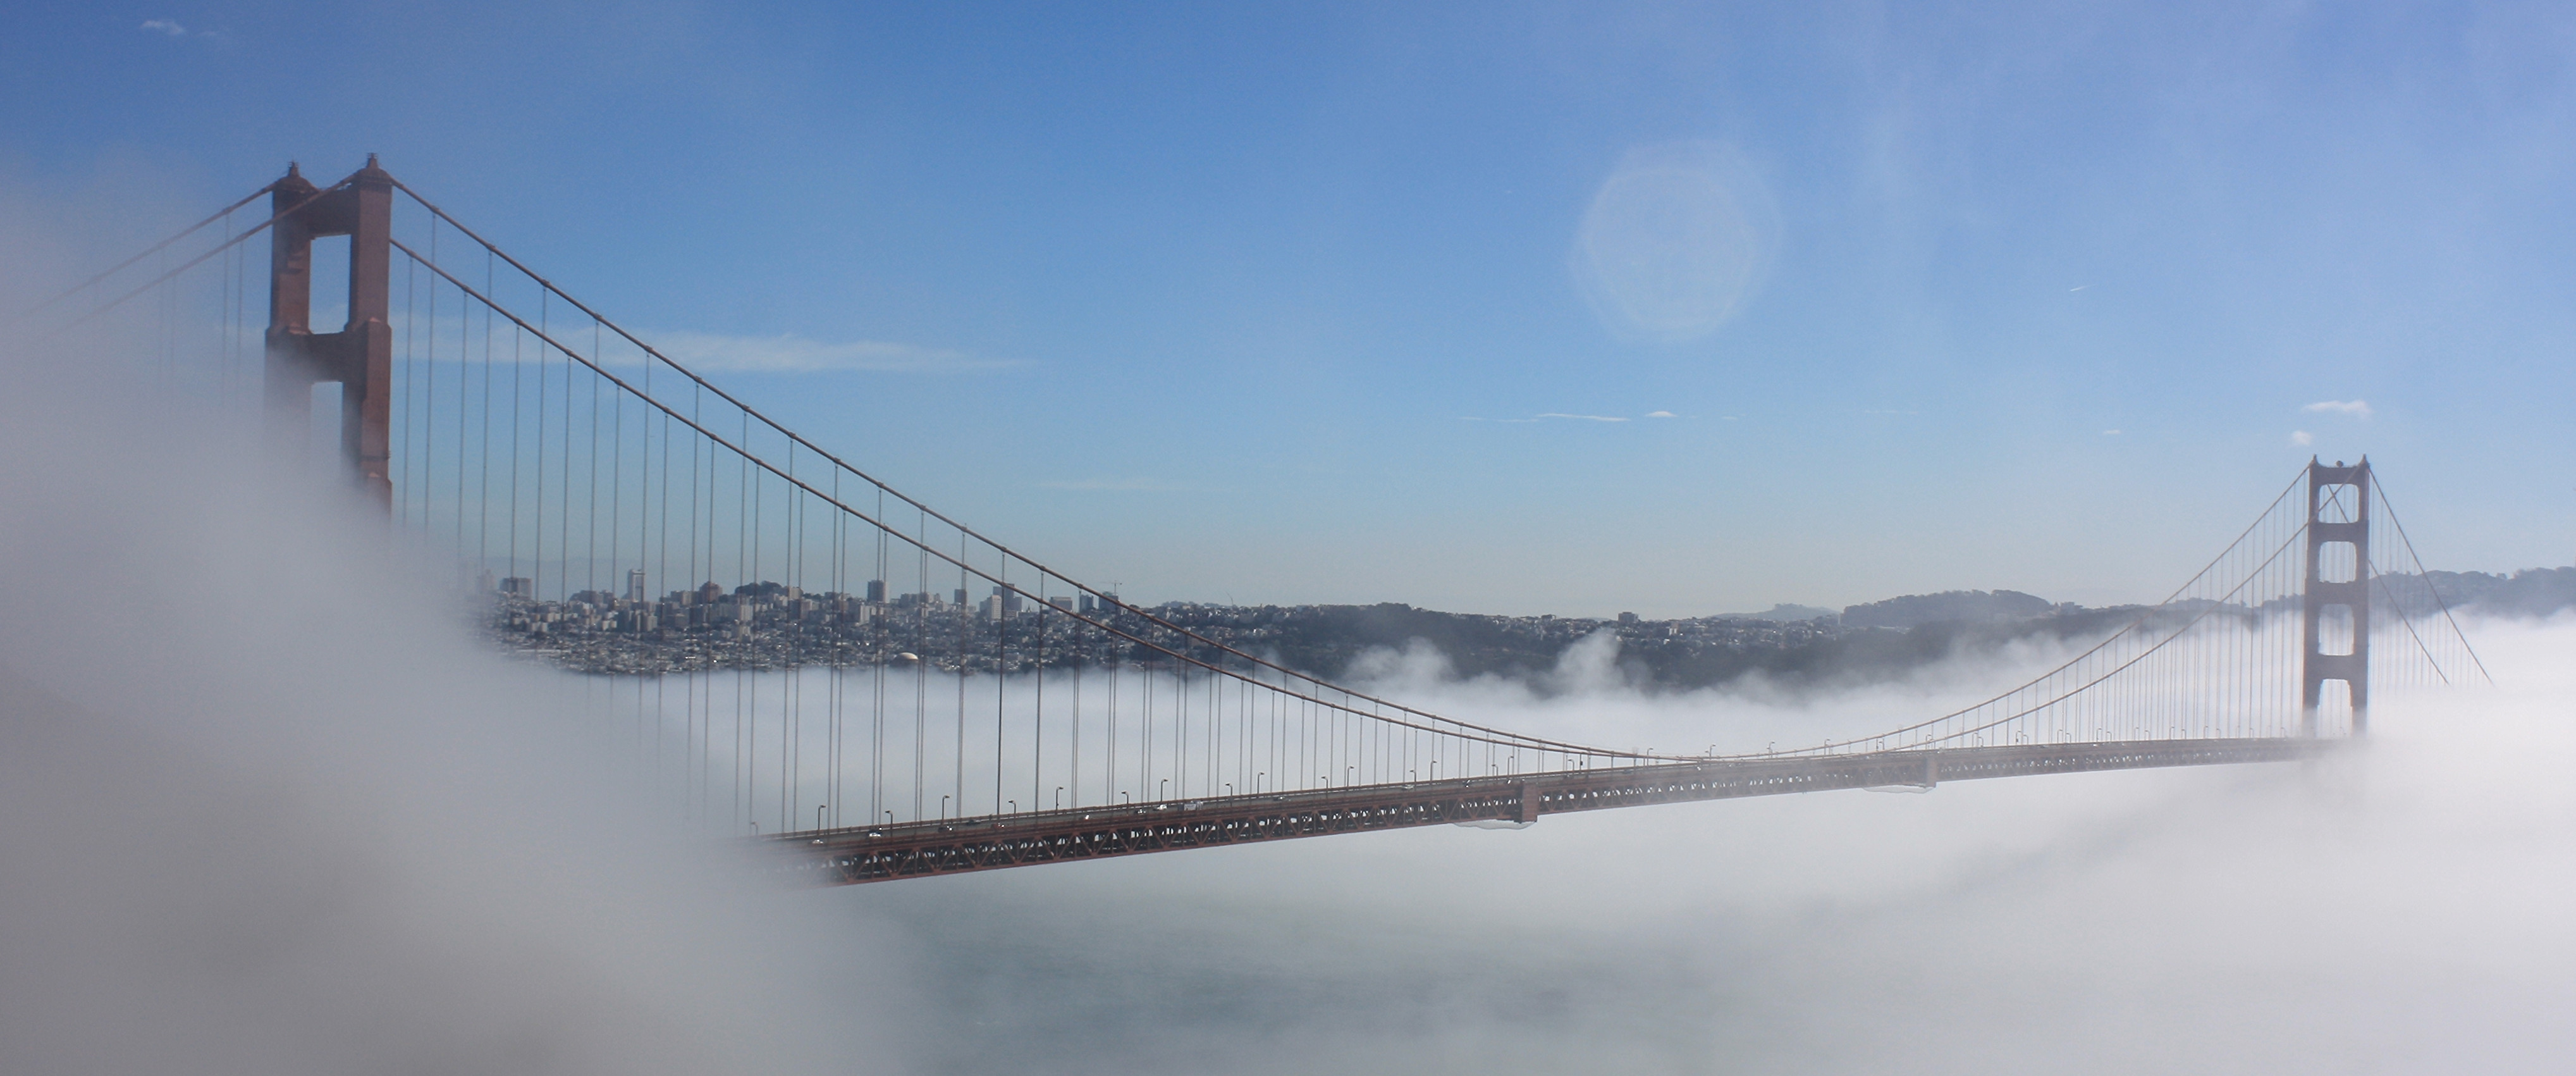
\includegraphics[width=0.9\textwidth]{figures/Golden_Gate_Bridge_by_Mark_Gunn.jpg} 
\end{center}
\end{frame}




\end{document}